\chapter{Experiment}
\label{sec:experiment}
In this section, the qualitative and quantitative performances of the proposed method are introduced. In this experiment, the empirical parameters as $\alpha=0.007$, $\beta=0.001$, $\lambda=0.25$, $\epsilon=10^{-2}$ are set. In addition, the proposed method is performed on Python implementation on PC with 16GB RAM, Intel Core i7-6700 CPU @ 3.40GHz. The test images come from the dataset provided in \cite{wvm}, \cite{rrm}, \cite{jiep}. Fig. \ref{fig:dataset} shows the 8 images tested in the experiments.
% ----Datasetの図----%
\begin{figure}[tb]
	\centering
	\includegraphics[width=1.0\hsize]{images/experiment/dataset.eps}
	\caption{These images used in the experiments.} \label{fig:dataset}
\end{figure}

\section{Comparison of Decomposition} \label{sec:decomposition}
The aim of the section is to evaluate how accurately the proposed method decomposes an observed image into the reflectance and illumination. As described in \cite{retinex}, the illumination should not distort the structure information while keeping smoothness. On the other hand, the reflectance should contain rich detail of an observed image. Although it is necessary to evaluate how much the proposed method estimates their component upon considering their characteristics, the ground truth for their component is difficult to obtain. Therefore, in order to confirm the effectiveness of the proposed method, the proposed method is compared with several state-of-the-art methods: three Retinec-based methods which are implemented in HSV-color space as well as the proposed method, including simultaneous reflectance and illumination estimation (SRIE) \cite{srie}, a weighted variational model (WVM) \cite{wvm}, and a joint intrinsic-extrinsic prior (JieP) \cite{jiep}. The codes of the three methods are downloaded from the author's Github websites and performed with recommended experimental settings.\par
Fig. \ref{fig:decoposition} summarizes the decomposition result of the reflectance and illumination from an observed image. SRIE and WVM cannot sufficiently distinguish between reflectance and illumination component, so that the estimated reflectance contains much illumination component. Moreover, the estimated illumination breaks the structure of the scene because it is over-smoothed. JieP significantly removes the illumination component from the reflectance, but the estimated illumination loses the meaningful structure information too much. In summary, 

\begin{figure*}[t]
\centering
	\begin{minipage}[b]{0.49\hsize}
		\centering
		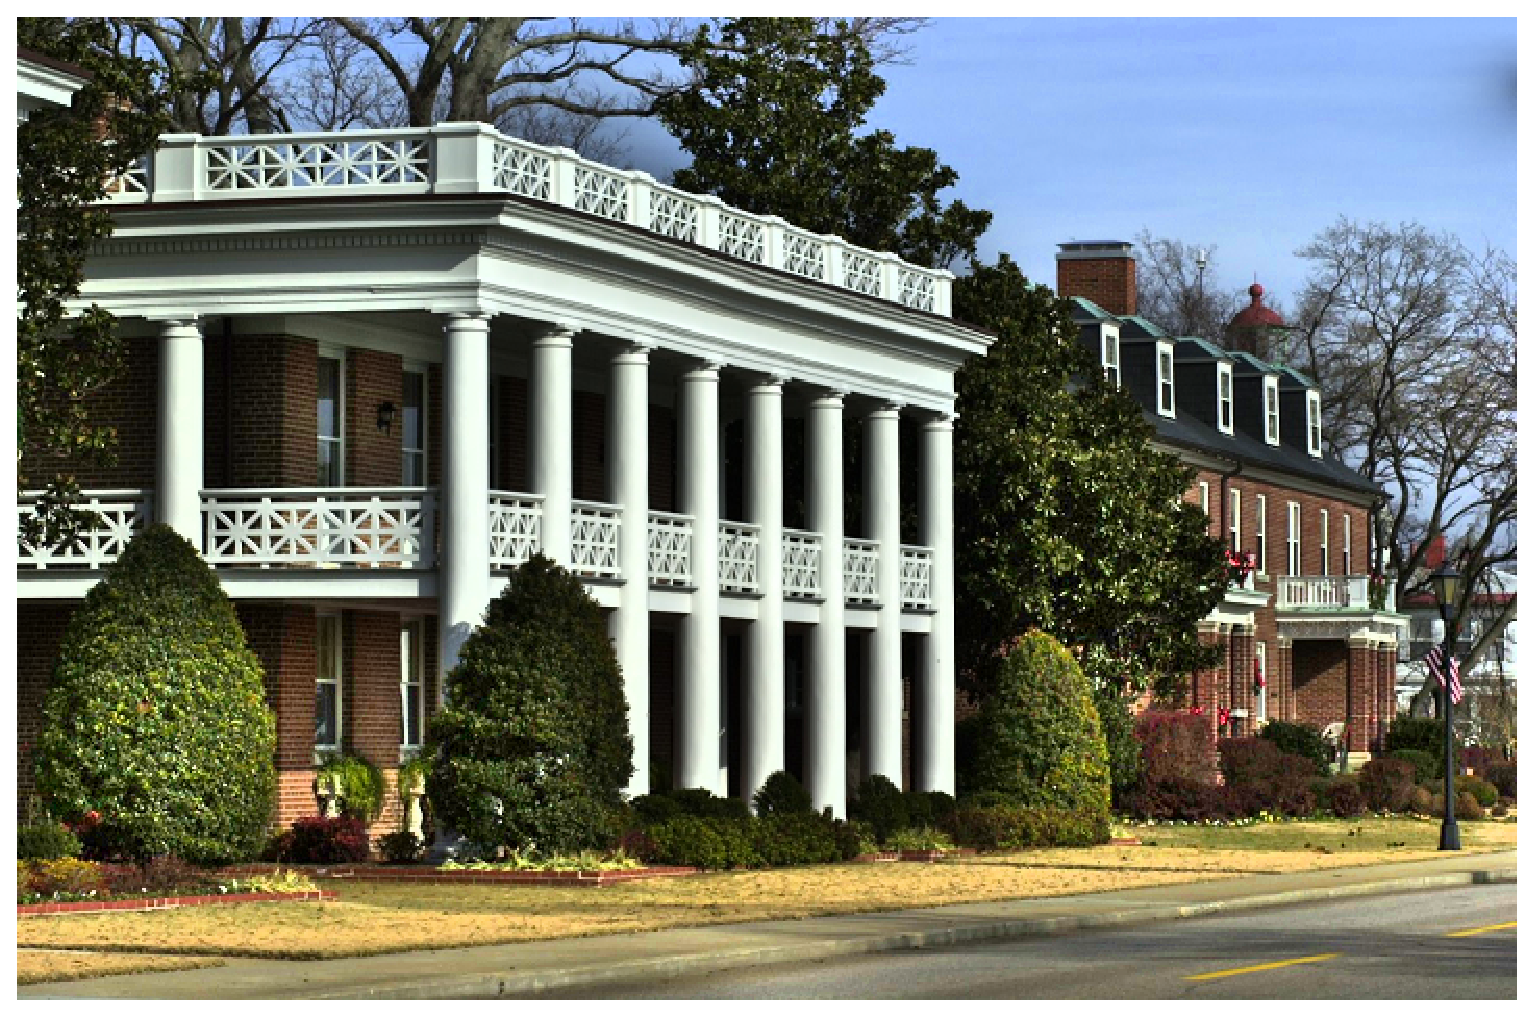
\includegraphics[width=72mm, height=48mm]{images/experiment/decomp/srie/reflectance.eps}
	\end{minipage}
	\begin{minipage}[b]{0.49\hsize}
		\centering
		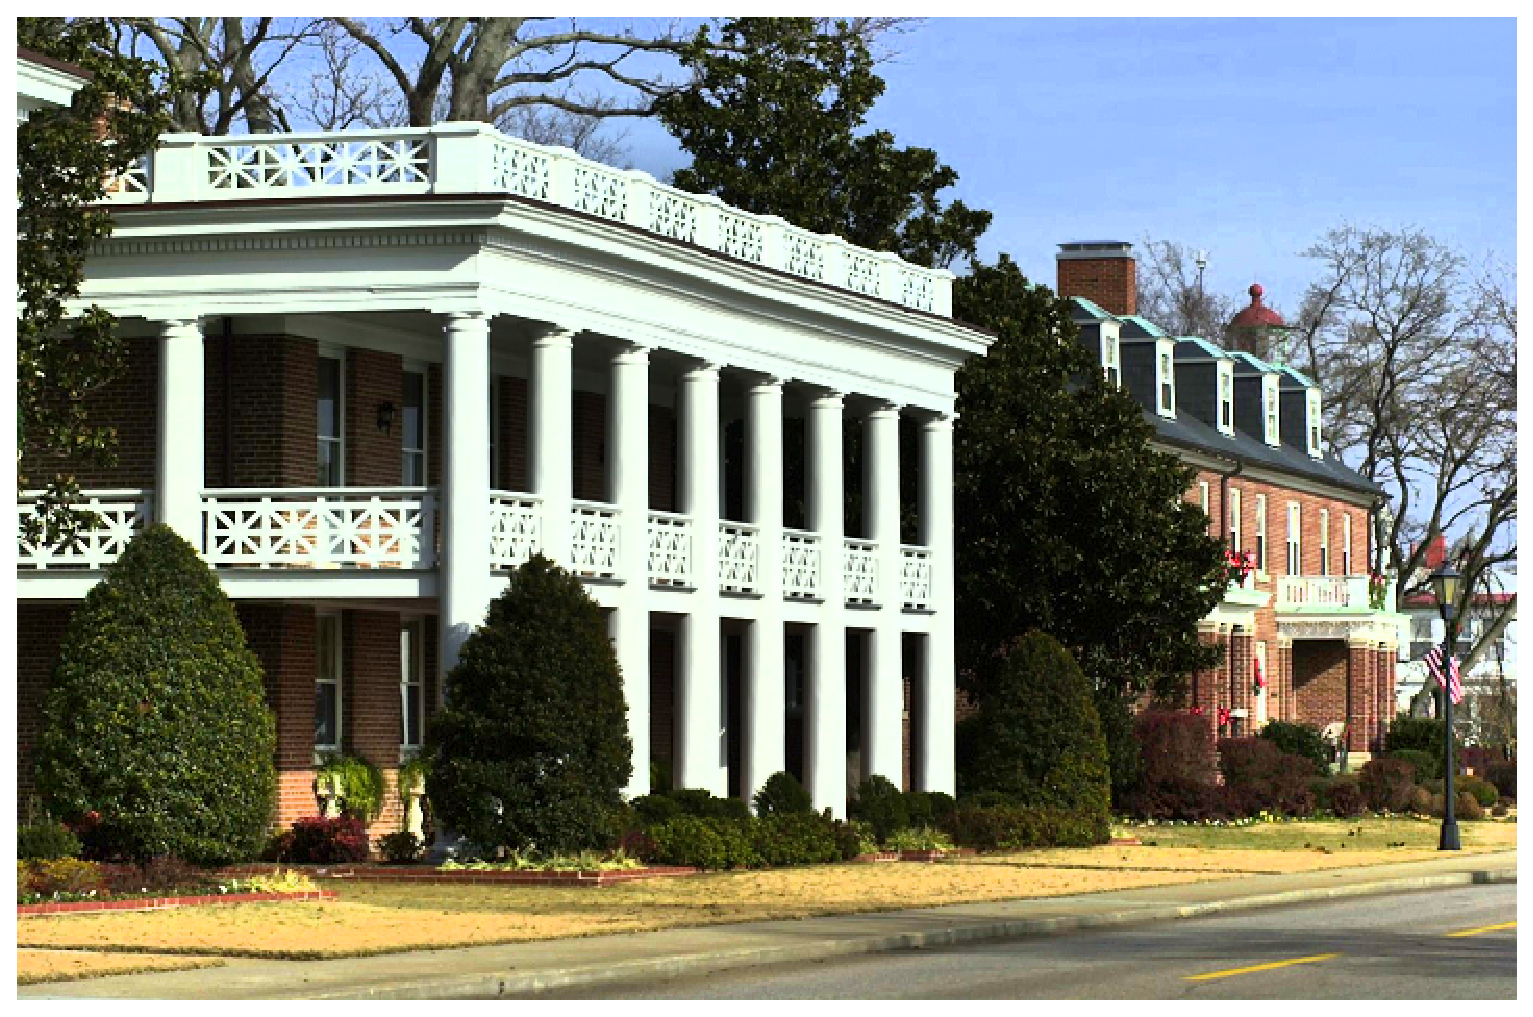
\includegraphics[width=72mm, height=48mm]{images/experiment/decomp/wvm/reflectance.eps}
	\end{minipage} \\
	\vspace{1.5mm}
	\begin{minipage}[b]{0.49\hsize}
		\centering
		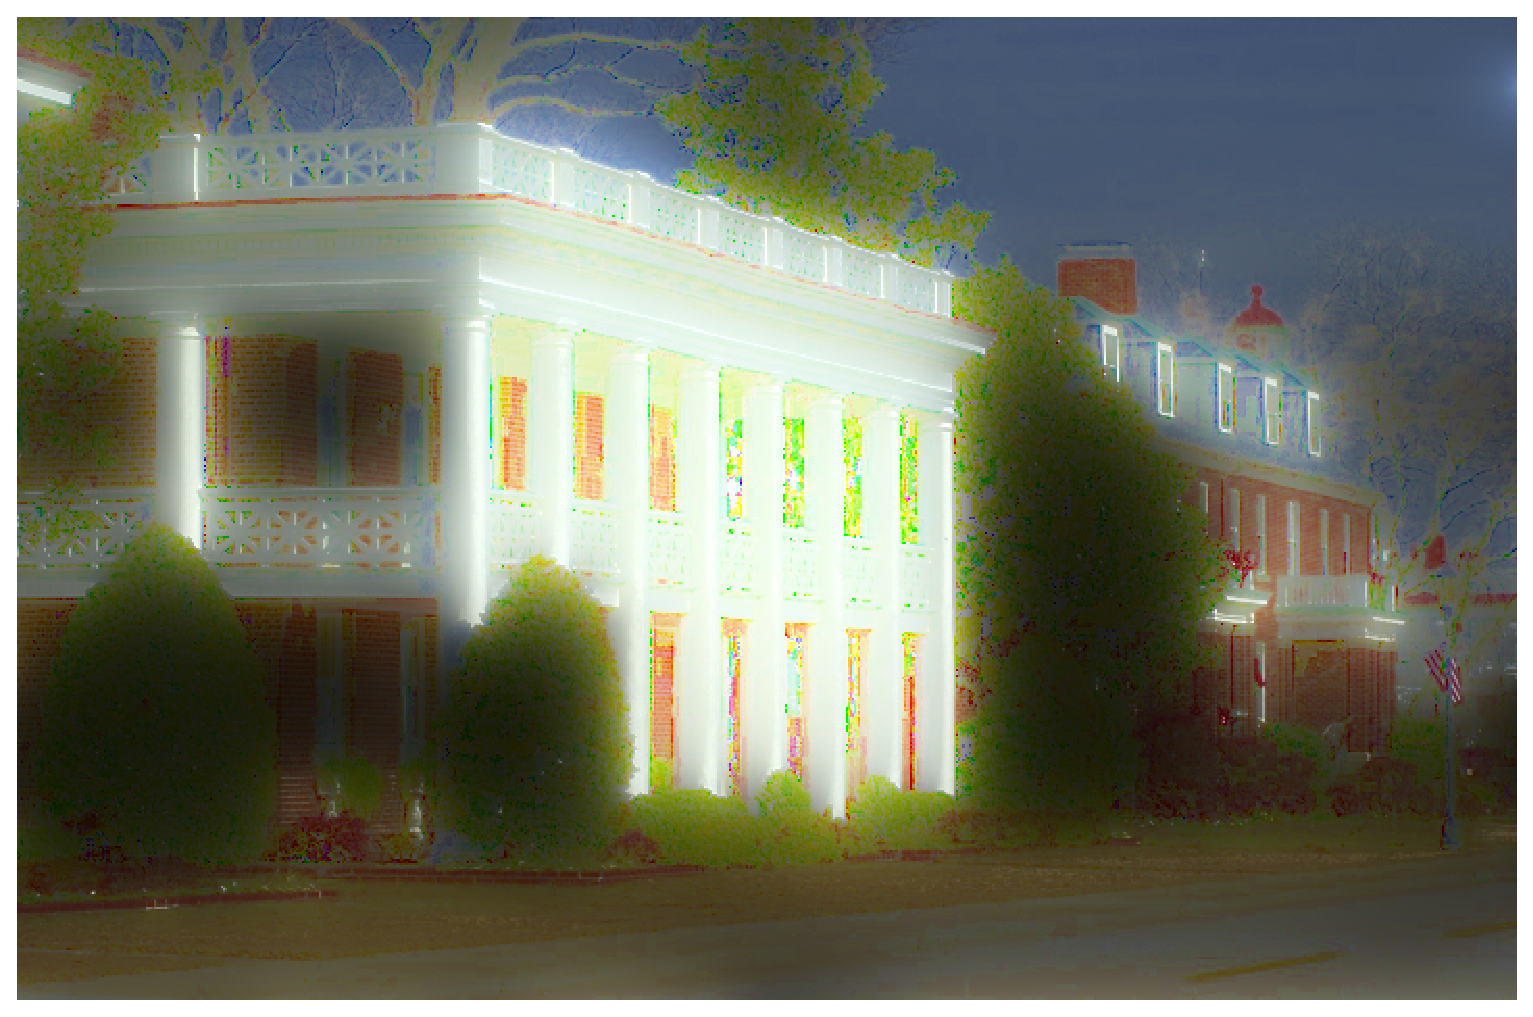
\includegraphics[width=72mm, height=48mm]{images/experiment/decomp/srie/illumination.eps}
		\subcaption{SRIE} \label{fig. decomp_srie}
	\end{minipage}
	\begin{minipage}[b]{0.49\hsize}
		\centering
		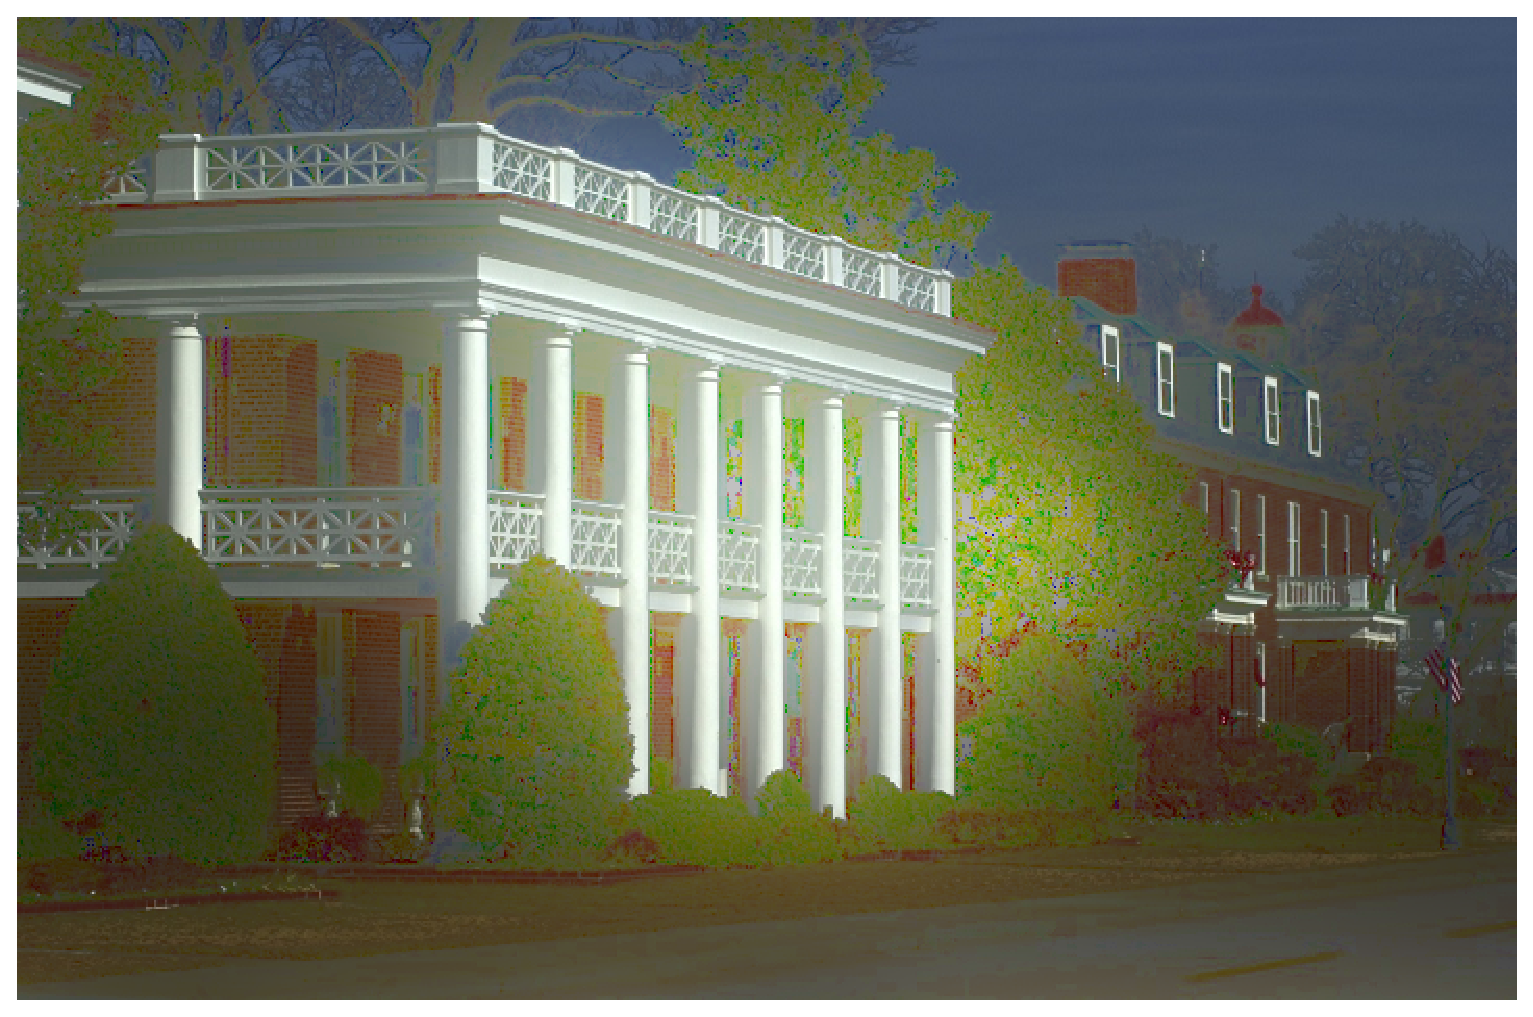
\includegraphics[width=72mm, height=48mm]{images/experiment/decomp/wvm/illumination.eps}
		\subcaption{WVM} \label{fig. decomp_wvm}
	\end{minipage}\\
	\begin{minipage}[b]{0.49\hsize}
	\centering
	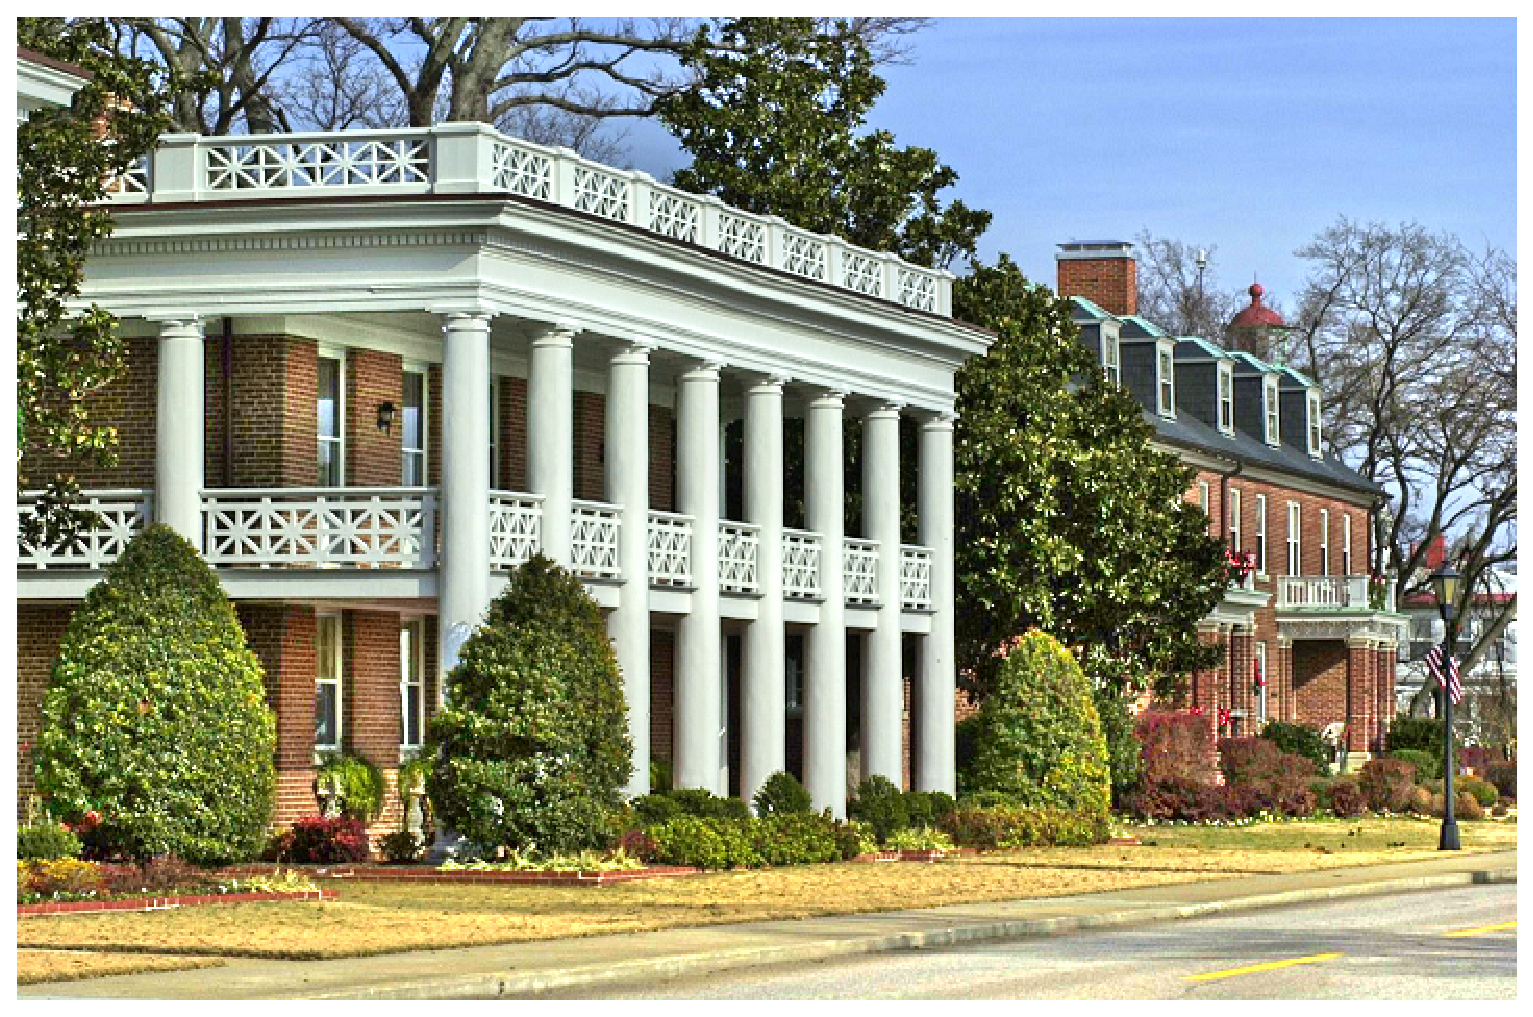
\includegraphics[width=72mm, height=48mm]{images/experiment/decomp/jiep/reflectance.eps}
	\end{minipage}
	\begin{minipage}[b]{0.49\hsize}
	\centering
	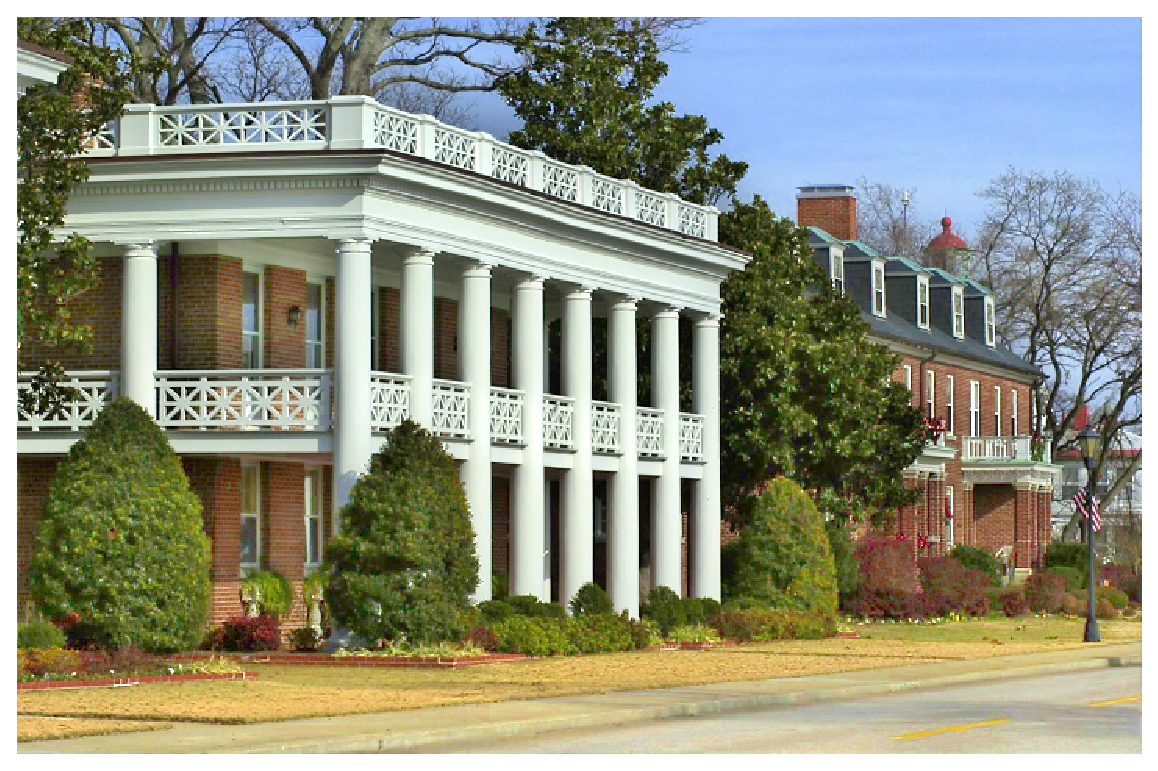
\includegraphics[width=72mm, height=48mm]{images/experiment/decomp/prop/reflectance.eps}
	\end{minipage}\\
	\vspace{1.5mm}
	\begin{minipage}[b]{0.49\hsize}
	\centering
	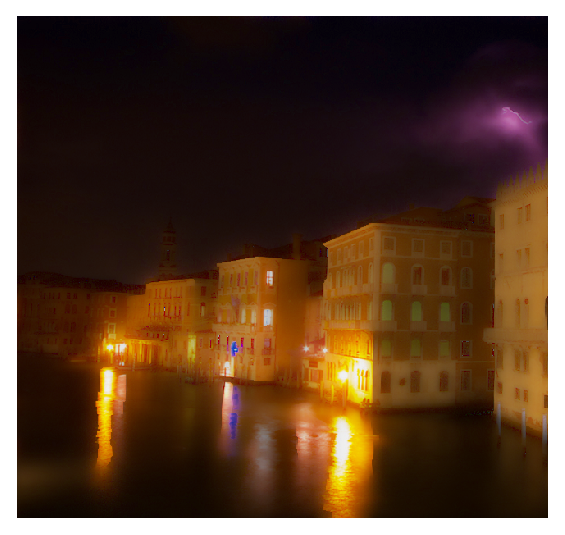
\includegraphics[width=72mm, height=48mm]{images/experiment/decomp/jiep/illumination.eps}
	\subcaption{JieP} \label{fig. decomp_jiep}
	\end{minipage}
	\begin{minipage}[b]{0.49\hsize}
	\centering
	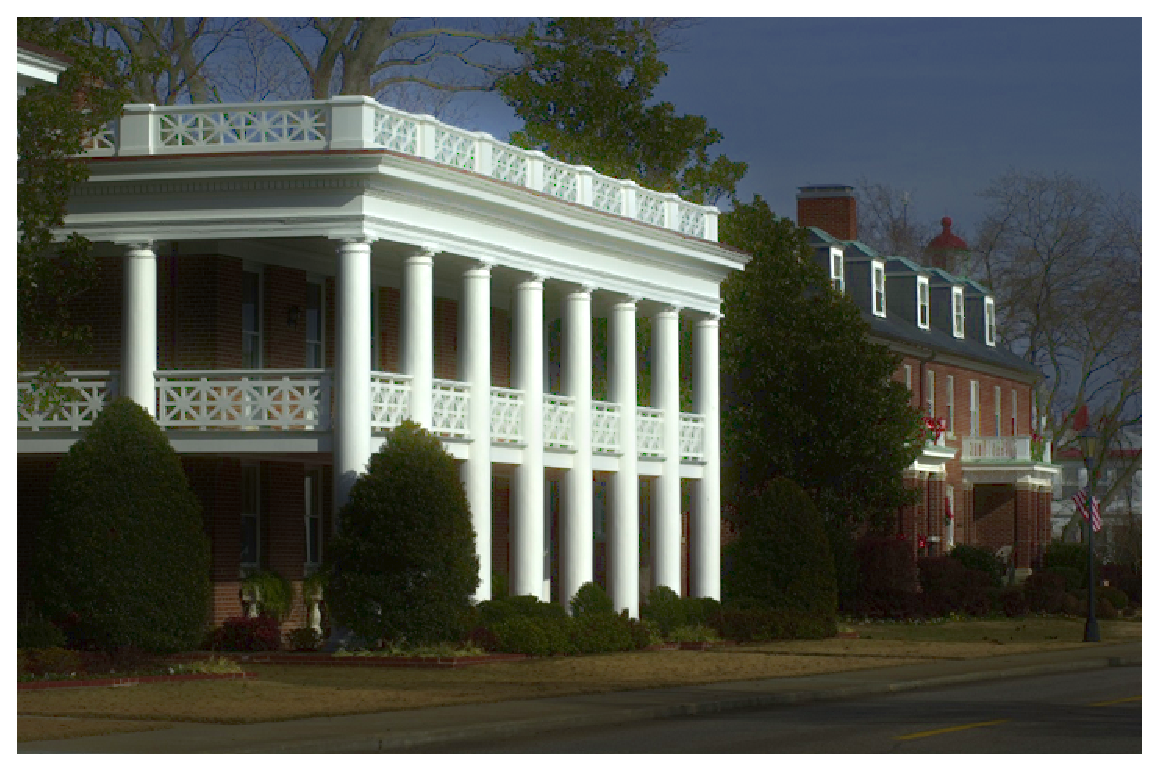
\includegraphics[width=72mm, height=48mm]{images/experiment/decomp/prop/illumination.eps}
	\subcaption{Ours} \label{fig. decomp_prop}
	\end{minipage}
	\caption{Reflectance and illumination decomposed by SRIE, WVM, JieP, and Ours. ((a)-(d) top: reflectance, bottom: illumination)}
	\label{fig:decomposition}
\end{figure*}